\documentclass[12pt,a4paper]{report}
\usepackage{fontspec}
\usepackage[vietnamese]{babel}
\usepackage{geometry}
\usepackage{amsmath}
\usepackage{amssymb}
\usepackage{graphicx}
\usepackage{tocloft}
\usepackage{float}

\setmainfont{Libertinus Serif}
\geometry{left=2cm, right=2cm, top=2cm, bottom=2cm}

\setcounter{tocdepth}{1}
\renewcommand{\cftchapfont}{\bfseries\Large}
\renewcommand{\cftsecfont}{\normalsize}

\begin{document}
\begin{titlepage}
	\centering
	\vspace*{2cm}
	
	{\LARGE\bfseries TRƯỜNG ĐẠI HỌC KHOA HỌC TỰ NHIÊN\\[0.3cm]
		KHOA TOÁN - CƠ - TIN HỌC\\[0.5cm]}
	
	\begin{figure}[H]
		\centering
		\IfFileExists{../../../../../LOGOHUS.png}{
			\includegraphics[width=0.3\linewidth]{../../../../../LOGOHUS.png}
		}{
			\IfFileExists{../../../../../LOGOHUS.jpg}{
				\includegraphics[width=0.3\linewidth]{../../../../../LOGOHUS.jpg}
			}{
				\fbox{LOGO HUS}
			}
		}
	\end{figure}
	
	{\huge\bfseries BÁO CÁO MINI-PROJECT\\[0.5cm]
		MÔN: THỊ GIÁC MÁY TÍNH (MAT3562E 2)\\[0.5cm]}
	
	{\Large\bfseries LAB 04 + 05}
	
	\begin{flushleft}
		{\large
			Giảng viên: TS. Cao Văn Chung\\
			Sinh viên: Bùi Quang Chiến\\
			MSSV: 23001837\\
			Lớp: MAT3562E 2\\
		}
	\end{flushleft}
	
	\vfill
	
\end{titlepage}

\tableofcontents
\newpage


\chapter{Lab 04: Biến đổi Hình học 2D (Geometric Transformations)}

\section{Công thức toán học và Trực quan hóa kết quả}
Các phép biến đổi hình học cơ bản bao gồm Tịnh tiến, Co giãn, Xoay và Xô lệch. Dưới đây là minh họa đầu ra đối với các phép biến đổi áp dụng trên ảnh.

\begin{figure}[H]
    \centering
    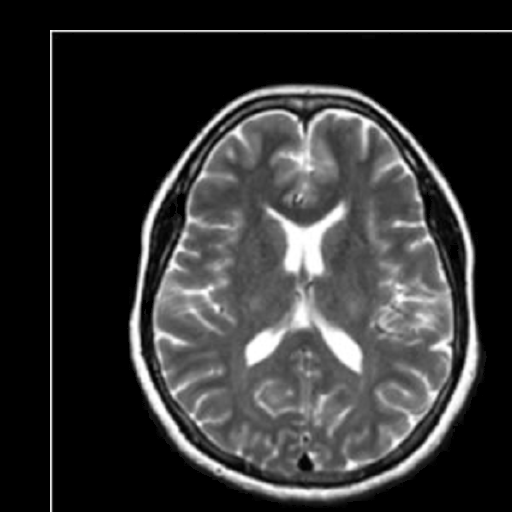
\includegraphics[width=0.7\textwidth]{data/translation_output.png} 

    \caption{Kết quả phép tịnh tiến (Translation)}
\end{figure}

\begin{figure}[H]
    \centering
    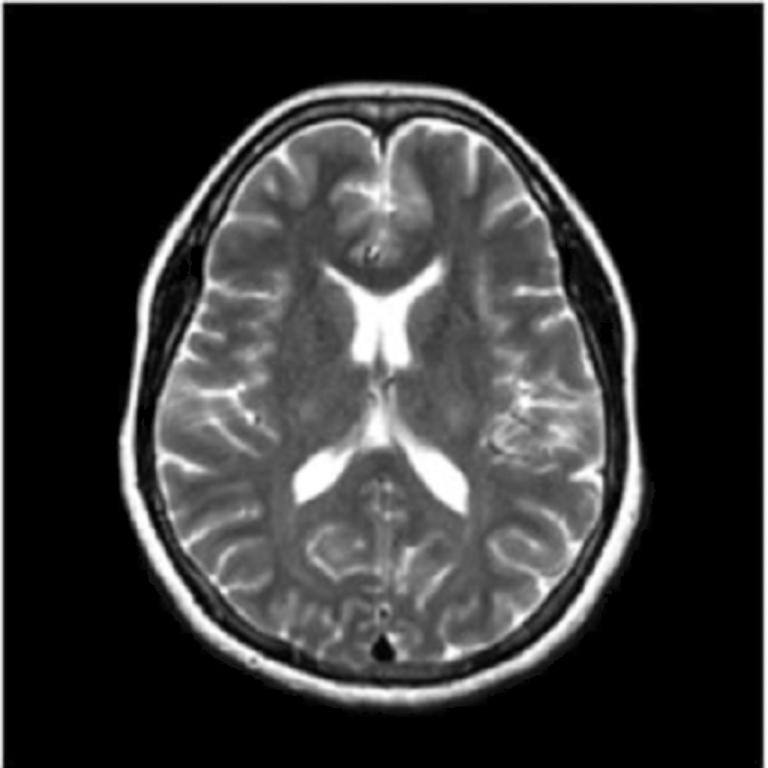
\includegraphics[width=0.7\textwidth]{data/scaling_output.png}

    \caption{Kết quả phép co giãn (Scaling)}
\end{figure}

\begin{figure}[H]
    \centering
     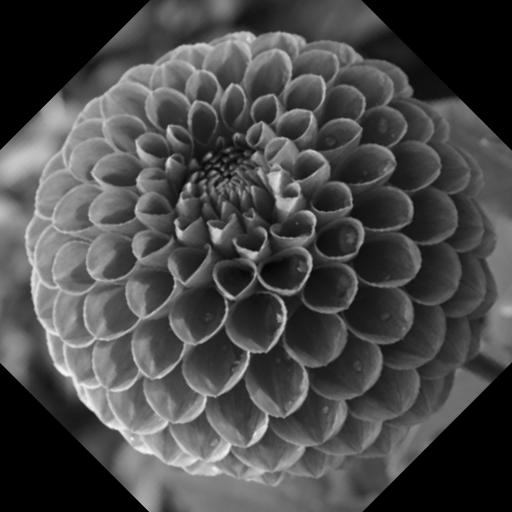
\includegraphics[width=0.7\textwidth]{data/rotation_output.png}

    \caption{Kết quả phép xoay (Rotation) và hiện tượng cắt viền (nếu có)}
\end{figure}

\section{Ánh xạ tiến (Forward) và Ánh xạ ngược (Inverse Mapping)}
Quá trình duyệt tại mỗi tọa độ $(x', y')$ của ảnh đích và tính ngược lại để dán điểm màu gốc tương ứng $(x, y)$ giúp khắc phục hoàn toàn hiện tượng tạo lỗ hở (holes) thường gặp trong ánh xạ tiến cơ sở.

\section{Tính giao hoán của Ma trận và Thứ tự phép}
Hoán đổi Xoay ($30^\circ$) rồi Xô lệch (Shear 1.5) so với Xô lệch (1.5) rồi Xoay ($30^\circ$): Hoàn toàn khác nhau về ngoại hình và phương trình biến đổi tịnh tính ($A \cdot B \neq B \cdot A$).
\begin{figure}[H]
    \centering
    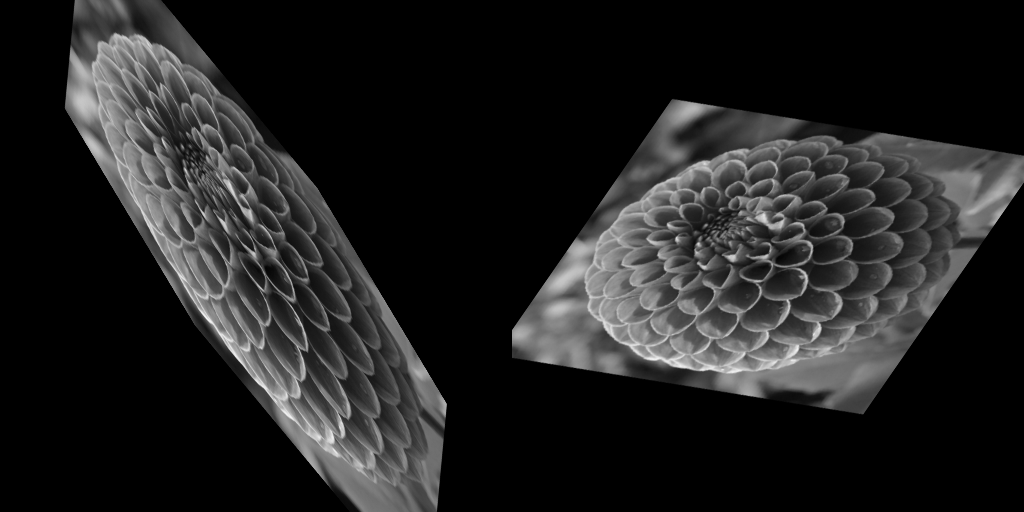
\includegraphics[width=0.8\textwidth]{data/order_comparison.png}

    \caption{Sự khác biệt khi hoán đổi thứ tự Xoay và Xô lệch}
\end{figure}

\section{So sánh Hiệu xuất: NumPy vs OpenCV}
Theo kết quả Benchmark từ hệ thống Python:
\begin{itemize}
    \item \textbf{Phép Tịnh tiến:} OpenCV ($\sim 1.02$ ms) vượt NumPy thủ công ($\sim 65.65$ ms) \textbf{64.3 lần}.
    \item \textbf{Phép Co giãn (1.5x):} OpenCV ($\sim 0.44$ ms) bỏ xa NumPy ($\sim 196.84$ ms) tới \textbf{445.7 lần}.
    \item \textbf{Phép Xoay ($45^\circ$):} OpenCV ($\sim 1.07$ ms) nhanh hơn NumPy ($\sim 199.76$ ms) khoảng \textbf{187.1 lần}.
\end{itemize}

\textit{Giải thích:} OpenCV tận dụng Backend C++, các nhánh vector SIMD phần cứng, kỹ xảo quản lý bộ nhớ để tránh khỏi delay của trình thông dịch Python.

\chapter{Lab 05: Tác vụ Hình thái học (Morphological Operations)}

\section{Hình thái học và Kết quả Tác vụ}
\begin{figure}[H]
    \centering
    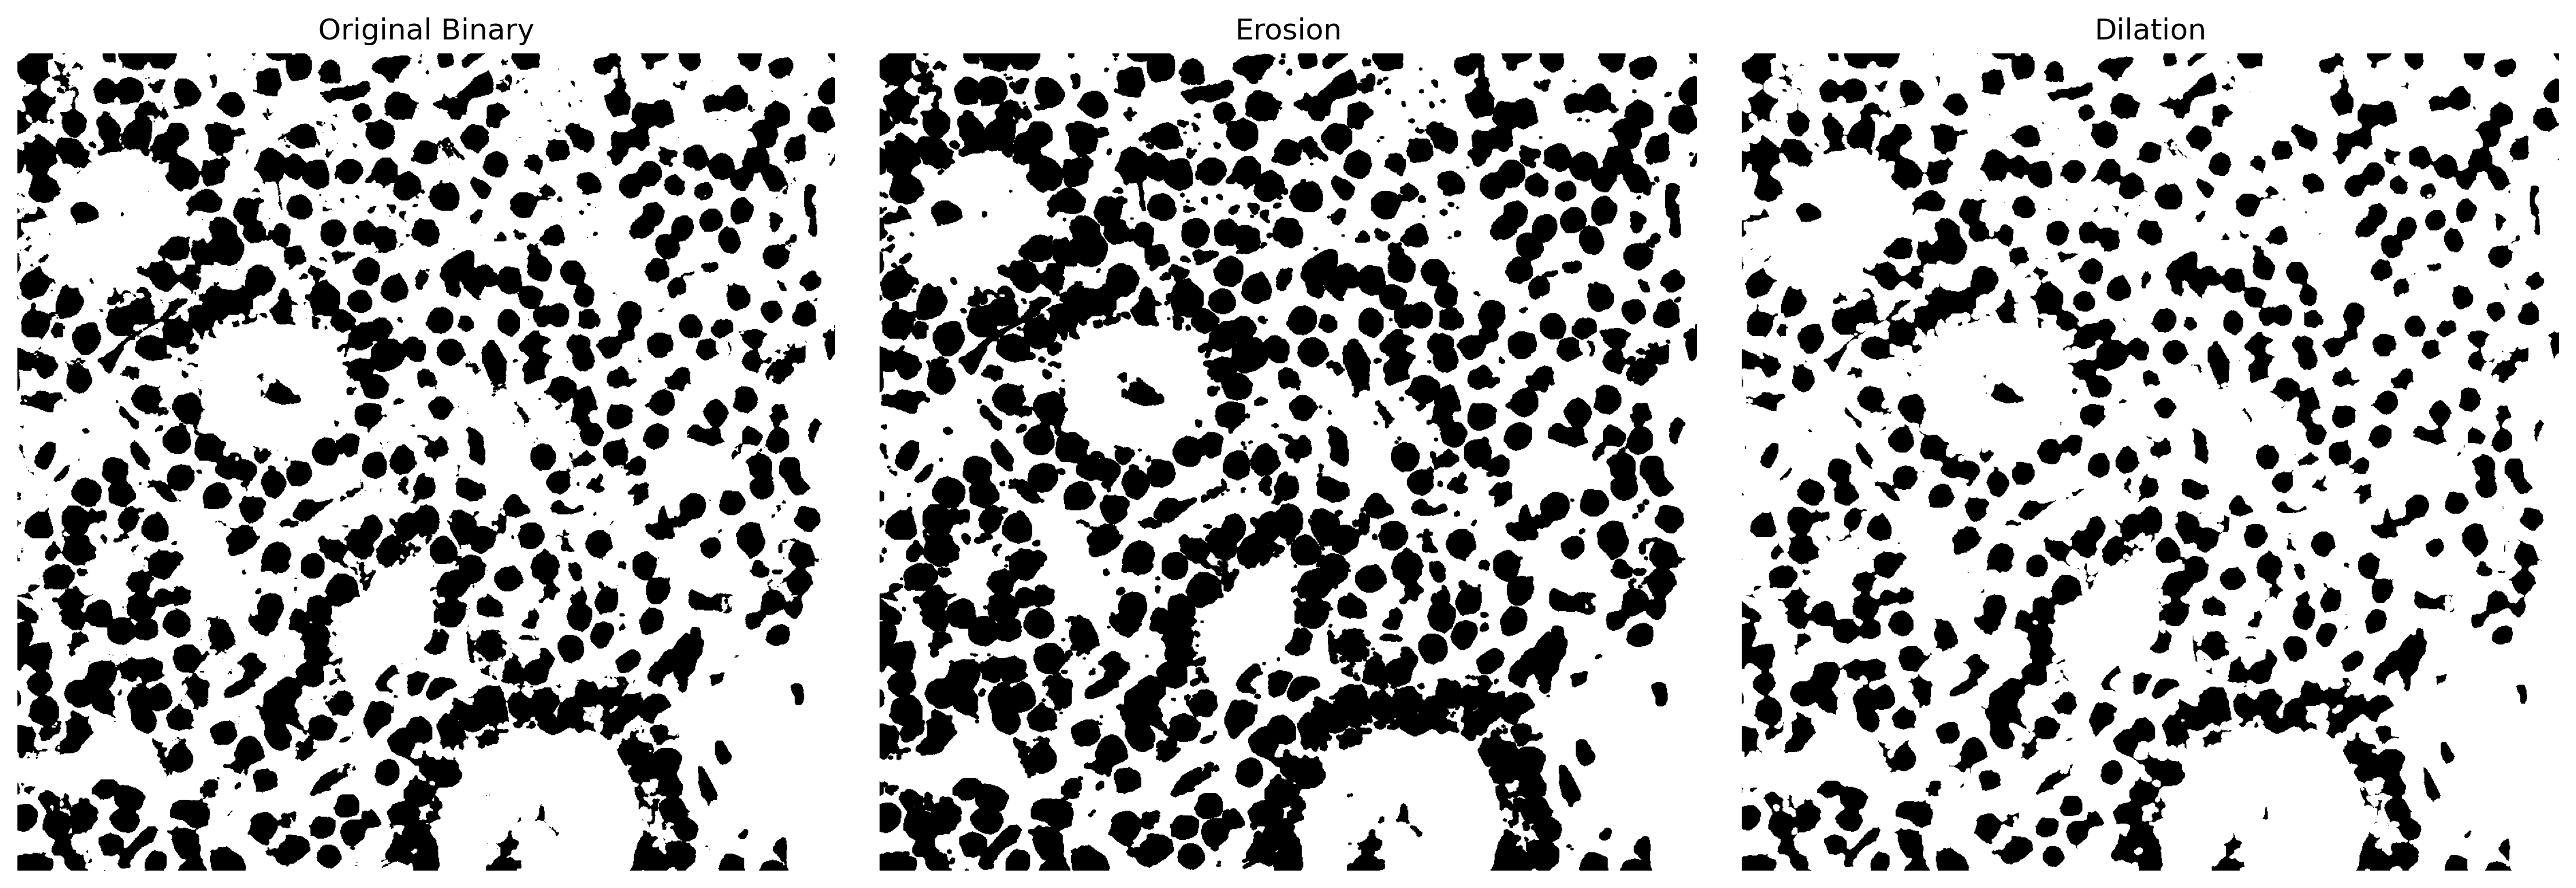
\includegraphics[width=0.8\textwidth]{data/erosion_dilation.png}

    \caption{Phép Co (Erosion) và Giãn (Dilation) trên ảnh cấu trúc}
\end{figure}

\begin{figure}[H]
    \centering
    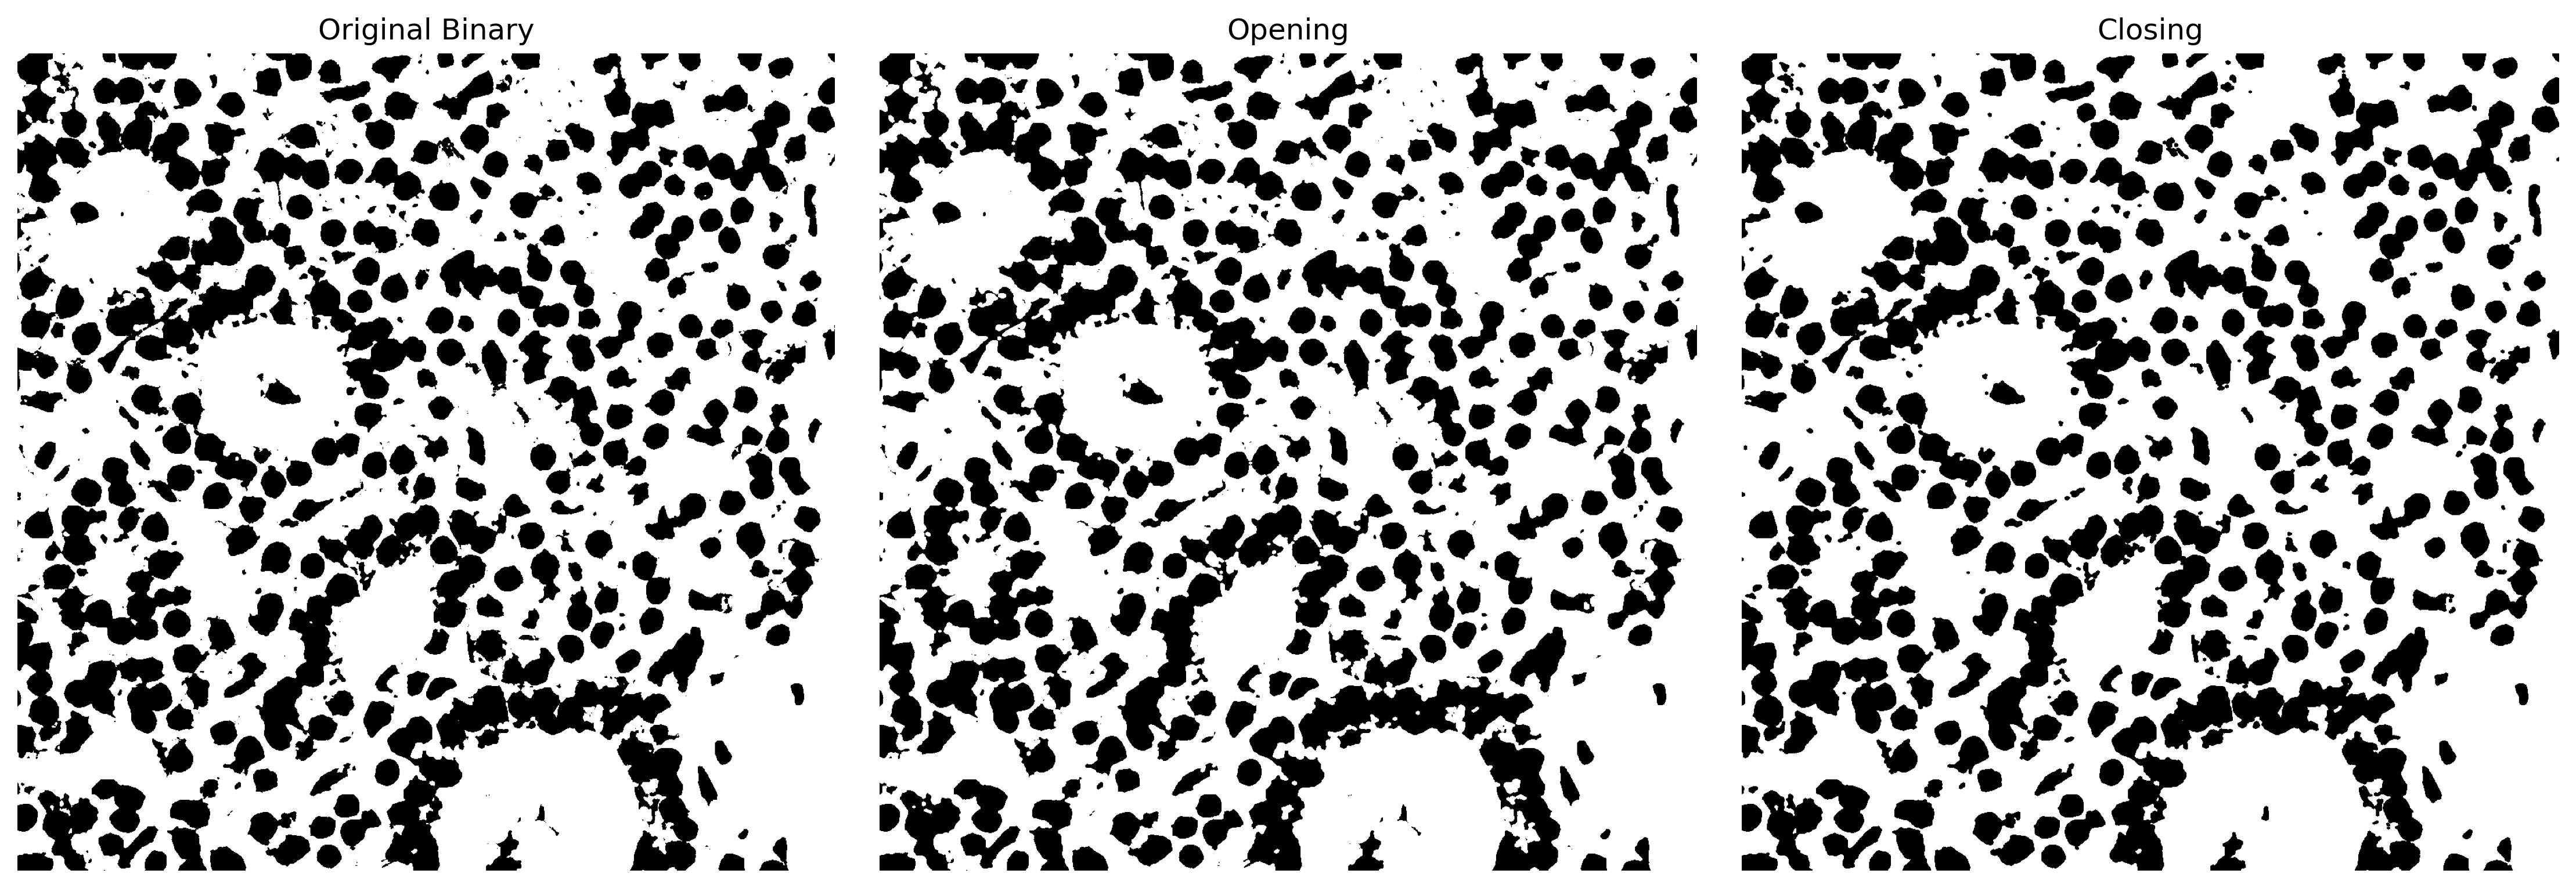
\includegraphics[width=0.8\textwidth]{data/opening_closing.png}

    \caption{Khử nhiễu với Opening và lấp lỗ nhỏ với Closing}
\end{figure}

\section{Bản chất toán học}
\subsection*{Co (Erosion) vs Giãn (Dilation)}
Erosion trích xuất cường độ cực tiểu tại khu vực (min), làm bào mỏng cung và phá gãy rãnh hẹp. Ngược lại, Dilation sử dụng cực đại lân cận (max), khâu và làm dày các nứt gãy hẹp.

\subsection*{Mở (Opening) và Đóng (Closing)}
Opening (Co rồi Giãn) triệt tiêu nhiễu gai sáng liti rải rác xung quanh nhưng vẫn giữ lại tổng viền. Closing (Giãn rồi Co) vá đầy rãnh nứt hay các đốm thủng tối nằm trong đối tượng.

\end{document}